% !TEX encoding = UTF-8 Unicode
% XeLaTeX can use any Mac OS X font. See the setromanfont command below.
% Input to XeLaTeX is full Unicode, so Unicode characters can be typed directly into the source.

% The next line tells TeX to typeset with xelatex, and to open and save the source with Unicode encoding.

% !TEX TS-program = xelatex

\documentclass[a4paper,twocolumn,12pt]{article}

% !TEX root = Time_Evo.tex

\usepackage{tocloft}
\renewcommand{\cfttoctitlefont}{\hfil \bfseries \sihao}
\renewcommand{\cftsecfont}{\bfseries \sihao}
\renewcommand{\cftsecpagefont}{\bfseries \sihao}
\renewcommand{\cftsubsecfont}{\bfseries \sihao}
\renewcommand{\cftsubsecpagefont}{\bfseries \sihao}
\renewcommand{\cftsubsubsecfont}{\bfseries \sihao}
\renewcommand{\cftsubsubsecpagefont}{\bfseries \sihao}

\usepackage{abstract}
\renewcommand{\abstractnamefont}{\sihao \bfseries}

\setlength{\cftbeforesecskip}{10pt}
\setlength{\cftbeforesubsecskip}{8pt}
\setlength{\cftbeforesubsubsecskip}{6pt}

\usepackage{titlesec}
\titleformat{\section}
  { \sihao \bfseries}
  {\thesection}{1em}{}
\titleformat{\subsection}
  { \sihao \bfseries}
  {\thesubsection}{1em}{}
\titleformat{\subsubsection}
  { \sihao \bfseries}
  {\thesubsubsection}{1em}{}  



\usepackage[retainorgcmds]{IEEEtrantools}
\usepackage{caption}
\usepackage{array}
\usepackage{setspace}
\usepackage{multicol}
\usepackage{multirow}
\usepackage{indentfirst}
\usepackage[font=small,labelfont=bf]{caption}
\setlength\parindent{0.85cm}
\setlength{\columnsep}{0.7cm}
\setlength{\parskip}{5pt}
\usepackage{pdfpages}
\usepackage{xcolor,graphicx}
\usepackage[hmargin=2.2cm,vmargin=2.5cm]{geometry}
\usepackage{makeidx}
\usepackage{amsmath,amsthm}
\usepackage[retainorgcmds]{IEEEtrantools}
\renewcommand\refname{参考文献}
\renewcommand\abstractname{摘要}
\renewcommand\tablename{表}
\renewcommand\figurename{图}
\renewcommand\contentsname{目录}
\renewcommand{\baselinestretch}{1.2}
\newcolumntype{P}[1]{>{\centering\arraybackslash}p{#1}}
\makeindex

%-----------------------------CJK Font Setup------------------------------!

\usepackage[PunctStyle=kaiming,AutoFakeBold=false,AutoFakeSlant=false,indentfirst,CJKnumber]{xeCJK}
\xeCJKDeclareSubCJKBlock{PUNC}{"FF1F}
\setCJKmainfont[BoldFont={Songti SC Bold}, PUNC=SimSun] {Songti SC Light}
\setCJKsansfont[BoldFont={Heiti SC Medium}]{Heiti SC}
\setCJKmonofont[BoldFont={Hiragino Sans GB W6}]{Hiragino Sans GB W3}

\setCJKfamilyfont{zhxinsong}{SimSun}
\setCJKfamilyfont{zhsong}[BoldFont={Songti SC Bold}]{Songti SC Light}
\setCJKfamilyfont{zhhei}[BoldFont={Heiti SC Medium}]{Heiti SC}
\setCJKfamilyfont{zhfs}{FangSong}
\setCJKfamilyfont{zhkai}[BoldFont={Kaiti SC Bold}]{Kaiti SC Regular}
\setCJKfamilyfont{zhli}{LiSu}
\setCJKfamilyfont{zhyou}{YouYuan}

\newcommand*{\simsun}{\CJKfamily{zhxinsong}} % 新宋
\newcommand*{\songti}{\CJKfamily{zhsong}}    % 宋体
\newcommand*{\heiti}{\CJKfamily{zhhei}}      % 黑体
\newcommand*{\fangsong}{\CJKfamily{zhfs}}    % 仿宋
\newcommand*{\kaishu}{\CJKfamily{zhkai}}     % 楷书
\newcommand*{\lishu}{\CJKfamily{zhli}}       % 隶书
\newcommand*{\youyuan}{\CJKfamily{zhyou}}    % 幼圆

% Use Fontsize inside {}, include a \par at the end of bracket to enable baselineskip
\newcommand{\chuhao}{\fontsize{42pt}{50.4pt}\selectfont}       %初号
\newcommand{\xiaochu}{\fontsize{36pt}{43.12pt}\selectfont}     %小初号
\newcommand{\yihao}{\fontsize{27.5pt}{33pt}\selectfont}        %一号
\newcommand{\erhao}{\fontsize{21pt}{25.2pt}\selectfont}        %二号
\newcommand{\xiaoer}{\fontsize{18pt}{21.6pt}\selectfont}       %小二号
\newcommand{\sanhao}{\fontsize{15.75pt}{18.9pt}\selectfont}    %三号
\newcommand{\sihao}{\fontsize{13.75pt}{16.5pt}\selectfont}     %四号
\newcommand{\xiaosi}{\fontsize{12pt}{14.4pt}\selectfont}       %小四号
\newcommand{\wuhao}{\fontsize{10.5pt}{12.6pt}\selectfont}      %五号
\newcommand{\xiaowu}{\fontsize{9pt}{10.8pt}\selectfont}        %小五号
\newcommand{\liuhao}{\fontsize{7.875pt}{9.45pt}\selectfont}    %六号
\newcommand{\qihao}{\fontsize{5.25pt}{6.3pt}\selectfont}       %七号

%----------------------------English Font Setup---------------------------!
\usepackage{fontspec,xltxtra,xunicode}
\defaultfontfeatures{Mapping=tex-text}
\setmainfont{Times New Roman}
\setsansfont[Scale=MatchLowercase,Mapping=tex-text]{Helvetica}
\setmonofont[Scale=MatchLowercase]{Times New Roman}

\newfontfamily{\AMT}{American Typewriter}
\newfontfamily{\Curly}{Baskerville}
\newfontfamily{\Fraktur}{Euclid Fraktur}


%Define Han Length
\newlength{\Han}
\settowidth{\Han}{汉}

%-------------------------------Language Setup----------------------------!

%-------------------------------Special Attention-------------------------!
\newsavebox{\myhbar}
\savebox{\myhbar}{$\hbar$}
\renewcommand*{\hbar}{\mathalpha{\usebox{\myhbar}}}


\begin{document}

\begin{titlepage}

  \includepdf{Book-Cover.pdf}

  \twocolumn[
  \begin{@twocolumnfalse}  
    \tableofcontents  
  \end{@twocolumnfalse}]
  
  \thispagestyle{empty}
  
\end{titlepage}

\pagestyle{fancy}
\chead{\xiaowu 复旦大学本科毕业论文}
\lhead{}
\rhead{}

\title{\sanhao \textbf{\heiti{波函数含时演化方法与性质研究\\
                       Time Propagation of Wave Functions }}}
\author{\xiaosi{\textbf{王逸群,李晔飞$^{\dagger}$}}}
\date{}

\twocolumn[
\begin{@twocolumnfalse}
  
  \maketitle

  \begin{abstract}
    \xiaosi
    % !TEX root = Time_Evo.tex

本课题构造了含时量子力学方法中使用的含时演化算符,其中使用了一维简谐振子的哈密顿量,并研究了不同波函数在该含时演化算符作用下的演化情况。我们使用$sinc$函数为基函数展开研究体系的波函数,并根据基函数的性质构造了一维简谐振子的哈密顿量在希尔伯特空间中的表示矩阵。切比雪夫展开法和对角化方法分别被用来展开含时演化算符,我们观察了不同的始态波函数的演化情况,对比了两种展开方法的数值表现。结果发现在我们所研究的小体系中切比雪夫展开和对角化方法在数值的表现几乎一致,因此在一定范围内可以相互验证彼此的稳定性与准确性。我们还研究了含时演化算符展开项表达式中的影响因素,如采样格点数,切比雪夫展开项数和时间步长等。目前看来含时演化算符的构造较为成功,下一步是优化所选用的基函数,改进哈密顿量中使用的近似方法,并利用含时演化算符模拟简单的拉曼光谱。

\bigskip
\noindent \textbf{关键词:\hspace{\Han}}
含时演化; \;
简谐振子; \;
切比雪夫展开; \;
对角化
  \end{abstract}
  
\renewcommand\abstractname{Abstract}
  \begin{abstract}
    \xiaosi
    % !TEX root = Time_Evo.tex

Time propagation operator in time-dependent quantum-mechanical methods was constructed with hamiltonian of one-dimensional harmonic oscillator system. Properties of time propagation of different systems under our operator have been studied. $sinc$ functions were set to be basis functionals, and hamiltonian matrix in Hilbert space was established accordingly. Chebyshev scheme and diagonalizatin method were used to represent the evolution operator, and we studied relevant factors such as sampling points, terms of Chebyshev expansion and time scale. We are going to use Fourier basis as well as better approximation methods to achieve higher precision, and try to calculate Raman Spectra with the time propagation operator. 

\bigskip
  \end{abstract}

\end{@twocolumnfalse}]

\clearpage
\xiaosi

\section{引言}
\label{sec:intro}
% !TEX root = Time_Evo.tex

化学变化是由反应体系内电子与原子核的运动和相互作用产生的,分子动力学的出现从微观上描述了化学反应的内部过程。基于第一性原理的理论计算为理论科学家的研究做出了长远的贡献。本论文主要讨论了如何用计算机程序模拟理论模型,将连续物理概念离散化处理等理论化学常规技术。关注的主要对象是求解含时薛定谔方程得到的波函数含时演化的性质,并尝试用简单的模型解释现实中的物理现象。理论计算的研究方法中最重要的两点性质包括算法的适应性和可移植性,所有算法耗费的计算资源都和体系的大小呈正相关关系,我们在相空间中研究并比较不同算法的适用性。由于计算资源和研究规模的限制,本课题选用的理论模型并不十分精确,因此主要是定性分析量子体系的性质;定量分析可以建立在正确的理论模型与更精确的数值方法的基础上。

近年来分子动力学快速发展,它的出现意味着物理化学研究从间接的宏观实验方法延伸到可以用理论模型模拟体系发生的过程。这样一来理论科学家们可以建立模型来研究孤立的基元反应,进而能对化学反应的微观过程有更深刻的认识。对基元反应的分离既可以从空间上做到,也可以从时间的维度完成。例如气固相表面的基元反应可以在高真空条件下将原子束轰击到表面上,可以视为空间上独立的反应;然而对于溶液中的基元反应,不能使用空间分离技术,可以通过超飞秒激光脉冲技术在时间尺度上分离反应。

在这里我们需要区分建立分子反应模型(modeling)和模拟分子反应体系(simulating)的概念。建模的目的是研究分子反应的微观机理,通过简单的计算验证一种可能的理论解释通常就足够了。而模拟反应的目的是定量地比较实验结果与理论预测情况。分子动力学模拟技术主要归功于计算机技术的发展和日益精确的实验研究方法。我们的课题主要涉及模拟反应体系,不过这一套理论工具同样适用于模型的建立。

基于第一性原理的主要量子力学理论方法有:
\begin{multicols}{2}
\begin{itemize}
  \item 经典轨迹法
  \item 半经典法
  \item 量子耦合法
  \item 含时量子方法
\end{itemize}
\end{multicols}
这些基本方法同时也是理论化学近似技术的理论基石。它们共同建立于波恩-奥本海默(Born-Oppenheimer)近似的假设上,即将原子核和电子的运动分开考虑。于是原子核的势能场就形成了电子运动和化学反应发生的势能面。




其中含时量子力学模型在分子动力学研究中有着重要的地位,其理论模型在计算机数值计算上易于实现性并且计算结果令人信服。含时模型的建立与发展基于含时薛定谔方程:
\begin{equation}
  i \hbar \frac{\partial \psi}{\partial t} = \hat{H} \psi  
\end{equation} 

从数值计算上来说,求解含时体系是一个初值问题,因此程序上容易实现。除此之外,其演化结果是直观可见的,可以有力地解释物理过程。通过引入含时哈密顿算符,含时算法还可以有效地描述受到外部作用的体系的演化情况,例如:体系在激光的作用下如何演化。本课题构建了一个一维简谐振子模型,用Chebyshev方法展开含时演化算符,研究其演化性质,并与其解析解进行比较。


\section{实验部分}
\label{sec:methods}
% !TEX root = Time_Evo.tex

\subsection{相空间和希尔伯特空间}
相空间和希尔伯特空间的概念对理解量子体系至关重要。

相空间(Phase Space)的概念在一定程度上统一了经典力学和量子力学。在经典力学中,相空间是一个表示系统所有可能状态的空间,它的每一个维度代表着体系的一个自由度。因此系统每个可能的状态在相空间中都对应着一个点。这里的状态并不仅仅包括体系内粒子的坐标$q$,还要考虑它们的速度或动量。一旦位置与动量确定后,我们可以根据牛顿力学预测体系下一步演化的信息。哈密顿方程描述了哈密顿量$H$关于时间$t$的演化关系:
\begin{equation*}
  \frac{d}{dt}q(t) = \frac{\partial H}{\partial p}(q(t),p(t))
\end{equation*}
\begin{equation*}
  \frac{d}{dt}p(t) = -\frac{\partial H}{\partial q}(q(t),p(t))
\end{equation*}

在量子力学中,众所周知量子态没有能准确描述的空间位置和动量信息。然而相空间和哈密顿量的物理概念还是存在的,体系的特定状态不再由相空间的一个点确定,而是以波函数的形式出现,由${\left|\Psi\right|}^2$概率分布决定状态。量子相空间的位置和动量算符成为了希尔伯特空间的厄米算符。每个量子力学量都对应着相空间里特定的波函数,反之亦然,即为量子力学量的本征态(Ref: Hermann Weyl and John von Neumann)。相空间中的本征值通过对角化希尔伯特空间中的表示矩阵得到,例如在本课题中,对角化哈密顿矩阵将得到一系列实数,它们是一维简谐振子各本征态的特征值。我们对物理现象的理解依赖于其连续性: 物理定律可以由连续函数描述。而量子计算模型建立于连续函数可被离散的采样点完全表示的基础上。在我们处理的量子力学体系中,相空间里最小的体积单元是$ h^{D} $(h是普朗克常数,D是体系的自由度)。这说明至少在每个体积单元中有一个采样点就可能离散地表示这个系统。相空间内的离散表示与波函数在希尔伯特空间里的表示密切相关。

希尔伯特空间(Hilbert Space)是带有内积的完备实或复向量空间。在希尔伯特空间V中定义内积:
\begin{equation}
  \left< f,g \right> = \int_a^b f(\tau)g(\tau)d{\tau}
\end{equation}
并且定义其模为:
\begin{equation*}
  \left| f \right| = \sqrt{\left< f,f \right>}
\end{equation*}
这样V便成为完备的度量空间。希尔伯特空间的内积和欧几里得空间中的点积形式非常相似,但其为连续积分的形式,因此希尔伯特空间是对欧几里得空间的一种拓展概念。希尔伯特空间将二维欧几里得平面和三维空间延拓到有穷或无穷维度的完备空间,并且适用微积分定理。量子力学的非定域性质使得我们必须找到一种离域的表示方法,在量子表示中使用的算符理论需要一个作用空间,例如含时演化算符和哈密顿算符都是作用在希尔伯特空间上的线性算符。希尔伯特空间允许定义非定域算符,因此为我们解决了这样的问题。希尔伯特空间的结构决定了相空间里的表示,下一节将具体描述希尔伯特空间里的表示方法。


\subsection{希尔伯特空间中的表示方法}
首先考虑这样一个问题,用有限个基函数来拟合任意一个波函数(一维空间):
\begin{equation}
  \Psi (x) \approx \sum_{i=1}^N c_i \phi_i (x)
\end{equation}
其中$\phi_i$构成一个标准正交基组,也就是说:
\begin{equation}
  \int_{-\infty}^{+\infty} \phi_i(x) \phi_j(x) dx = \delta_{ij}
\end{equation}
$\delta_{ij}$是Kronecker Delta符号。那么接下来问题变为如何求解展开项系数$c_i$。由基函数的正交性可以得到:
\begin{IEEEeqnarray}{rCl}
    \Psi (x) & = & \sum_{i=1}^N c_i \phi_i (x) \nonumber \\
    \Psi (x) \phi_j(x) & = & \sum_{i=1}^N c_i \phi_i(x) \phi_j(x) \nonumber \\
    \sum_{i=1}^{N}c_i \delta_{ij} & = & \int_{-\infty}^{+\infty} \Psi(x) \phi_j(x) dx \nonumber \\
    c_i & = & \int_{-\infty}^{+\infty} \Psi(x) \phi_i(x) dx
\end{IEEEeqnarray}
在狄拉克表示中,$c_i$可以表示为$\left< \phi_i | \Psi \right>$,也就是将$\Psi$投影到基函数$\phi_i$上。然而需要注意,在数学上简单成立的公式并不一定可以方便地由计算机实现。在数值计算时我们总希望使用离散的表示方法。为了实现离散化计算,我们将使N个采样点的展开项值等于解析解的值:
\begin{equation}
  \Psi (x_k) = \sum_{i=1}^N c_i \phi_i (x_k)
\end{equation}
$x_k$为采样格点。离散采样的基组满足正交归一性:
\begin{equation}
  \sum_{k=1}^{K} \phi_i(x_k) \phi_j(x_k) = \delta_{ij}
\end{equation}
同样由正交性可得:
\begin{IEEEeqnarray}{rCl}
    \Psi (x_k) & = & \sum_{i=1}^N c_i \phi_i (x_k) \nonumber \\
    \Psi (x_k) \phi_j(x_k) & = & \sum_{i=1}^N c_i \phi_i(x_k) \phi_j(x_k) \nonumber \\
    \sum_{i=1}^{N}c_i \delta_{ij} & = & \sum_{k=1}^K \Psi(x_k) \phi_j(x_k)  \nonumber \\
    c_i & = & \sum_{k=1}^{K} \Psi(x_k) \phi_i(x_k)
\end{IEEEeqnarray}
从后面的推导我们将会看到,这一组基函数的系数将构成一个矢量,希尔伯特空间内的算符操作矩阵将作用在波函数的系数矢量上。因此今后这组系数矢量将作为波函数的具体形式出现和使用。


\subsection{基函数的选择}\label{sec:basis}
如上所述,我们需要找到一组合适的基函数$\phi_i$来展开所研究体系的波函数。基函数需要拥有的性质包括正交归一性并满足一定的边界条件。当然了,非正交归一的基函数也可以工作,不过在后续处理时会引入重叠积分项。本课题选取的基函数是$sinc$函数,即:
\begin{equation}
  \phi_i(x) = \frac{sin[\pi(x-x_i)]}{\pi (x-x_i)}
\end{equation}
\begin{figure}[hbt]
  \center
  \vspace{-1mm}
  \includegraphics[width=0.95\linewidth]{Sinc}
  \caption{Sinc函数}
  \label{fig:Sinc}
\end{figure}
并且理想上认为$\phi_i(x)$当且仅当$x=x_i$时表达式值为1,其他情况为0。显然sinc函数满足正交归一的性质
从后面的推导我们将看出,在这里$\phi_i(x)$的具体表达式并不重要,不会影响后续的表示。

然而性质更好的基函数可以由傅里叶方法得到。傅里叶方法得意重用是由于它表明在单位体积相空间内取一个采样点是可实现的,并且快速傅里叶变换算法(FFT)在数值计算上有很大优势,其算法复杂度随着相空间的体积半线性增长。傅里叶方法中,基函数表达式为:
\begin{equation}
  \small{\phi_k(x) = e^{i 2 \pi k x / L}, k = -(N/2-1),...,N/2}
\end{equation}
其中采样点为等距节点: $x_j = (j-1) \Delta x$,N为采样点数,L是采样长度。波函数可以近似表示为:
\begin{equation}
  \Psi(x) \approx \sum_{k=-(N/2-1)}^{N/2} c_k e^{i 2 \pi k x / L}
\end{equation}
由傅里叶级数的正交性可得系数项:
\begin{equation}
  c_k = \frac{1}{N} \sum_{j=1}^{N} \Psi(x_j) e^{-i 2\pi k x_j /L}
\end{equation}
其系数项表示了波函数在动量空间里的振幅,有重要物理意义。

\subsection{哈密顿算符的表示}
离散希尔伯特空间的构建让我们能够表示定域和非定域的算符。量子力学中最重要的算符是哈密顿算符(Hamiltonian Operator),在我们表示哈密顿算符之前,先推导狄拉克表示下的算符性质。需要注意,任意波函数都由是一组由无穷多体系本征态的线性组合构成的,因此波函数的完全展开应该含有无穷多项。然而我们只能在计算机能力允许的条件下用有限个基函数拟合波函数。
令$\phi_i (i=1,2,…,n)$ 构成一组标准正交基,即:
\begin{equation}
  \left< \phi_i | \phi_j \right> = \delta_{ij}
\end{equation}
\begin{equation}
  \Sigma_j \left| \phi_j \left> \right< \phi_j \right| = I
\end{equation}
其中$I$为恒等算符。
\begin{IEEEeqnarray}{rCl}
  \hat{O} \left| \phi_i \right> & = & I \hat{O}\left| \phi_i \right> \nonumber \\
  & = & \Sigma_j \left| \phi_j \left> \right< \phi_j \right|\hat{O} \left| \phi_i \right>  \nonumber\\
  & = & \Sigma_j O_{ji}\left| \phi_j \right>
\end{IEEEeqnarray}

其中$O_{ij} = \left< \phi_i \left| \hat{O} \right| \phi_j \right>$,这样便将非定域的算符在希尔伯特空间的基组表示下构造出来,在计算机中进行矩阵的运算。下面将进一步描述构造的原理:
考虑将波函数由一系列基函数展开,$\left< \Psi \right> = \Sigma_i c_i \left| \phi_i \right>$,在基函数形式确定后,实际上只需要得到其系数矩阵C就可以表示波函数。因此往后我们使用矩阵C代表波函数的系数矩阵。展开式可以表示为:
\begin{equation}
  \left| \Psi \right> = \Sigma_i C_i \left| \phi_i \right>
\end{equation}
将算符$\hat{O}$作用于波函数:
\begin{IEEEeqnarray}{rCl}
  \hat{O} \left| \Psi \right> & = & \Sigma_i \hat{O} C_i \left| \phi_i \right> \nonumber\\
  & = & \Sigma_i \Sigma_j O_{ji} C_i \left| \phi_j \right> \nonumber\\
  & = & \Sigma_j \left( \Sigma_i O_{ji} C_i \right) \left| \phi_j \right> \nonumber\\
  & = & \Sigma_j {\left( OC \right)}_j \left| \phi_j \right>  
\end{IEEEeqnarray}
\indent 将(15)和(16)对比发现$\hat{O}$算符作用后相当于将我们构建的$O$矩阵左乘原系数矩阵。那么接下来我们就要找到哈密顿算符$\hat{H}$在我们选取的基组下的矩阵表示。\par
在简谐振子模型中哈密顿算符可以被分解为动能项和势能项两部分,分别记为$\hat{T}$和$\hat{V}$。在原子单位(a.u.)下可以表示为:
\begin{equation}
  \hat{H} = \hat{T} + \hat{V}
\end{equation}
\begin{equation}
  \hat{T}(p) = \frac{\hat{p}^2}{2\mu}
\end{equation}
\begin{equation}
  \hat{V}(x) = \frac{1}{2} k \hat{x}^2
\end{equation}
$\hat{p}$为动量算符,并且有$\hat{p} = -i\hbar \frac{\partial}{\partial x}$ ; $\mu$为体系的约化质量;$k$为体系的力常数。考虑动能项矩阵的元素:
\begin{IEEEeqnarray}{rCl}
  T_{ij} & = & \left< \phi_i \right| \hat{T} \left| \phi_j \right> \nonumber\\
  & = & \left< \phi_i \right| -\frac{1}{2\mu}\frac{\partial^2}{\partial x^2}\left| \phi_j \right> \nonumber\\
  & = & -\frac{1}{2\mu}\int_{-\infty}^{\infty} {\phi_i}^{*}\frac{\partial^2 \phi_j}{\partial x^2} dx \nonumber
\end{IEEEeqnarray}
动能项含有二阶导数计算,对此我们采用三点近似法(three-point-approximation)处理:
\begin{equation*}
  \frac{\partial^2 \phi_j}{\partial x^2} = \frac{\phi_j(x+\Delta x) + \phi_j(x-\Delta x) - 2\phi_j(x)}{{\Delta x}^2}
\end{equation*}
根据$sinc$函数的正交性质易知:
\begin{align}
  T_{ij} & = 
  \begin{cases}
    \frac{1}{\mu {\Delta x}^2} & i=j\\
    -\frac{1}{2\mu {\Delta x}^2} & \left| i-j \right| =1 \\
    0 & \small{\text{其他情况}}
  \end{cases}
\end{align}
同时对势能项采用定域近似,即体系的势能仅由所测量该位置的势能决定:
\begin{IEEEeqnarray}{rCl}
  V_{ij} & = & \left< \phi_i \right| \hat{V} \left| \phi_j \right> \nonumber\\
  & = & \left< \phi_i \right| \frac{1}{2}k x^2 \left| \phi_j \right> \nonumber \\
  & \approx & V(x_i) \cdot \delta_{ij} 
\end{IEEEeqnarray} \par
我们采用等距结点法,在$(-2,2)$区间上采100个样,并根据上述表达式构造出哈密顿算符的矩阵,显然这是一个$100*100$的方阵。经过对角化将得到的结果和理论预测相比较,见表\ref{tab:Hamiltonian}
\begin{table}[!ht]
  \centering
  \begin{tabular}{P{1cm}|P{1.7cm}|P{1.7cm}|P{1.8cm}}
    \hline
     $\nu$ & 理论值 & 计算值 & 相对误差 \\ \hline
     1 & 3.1416 & 3.1396 & 0.06\%                   \\ \hline
     2 & 9.4248 & 9.4149 & 0.15\%                   \\ \hline
     3 & 15.7080 & 15.6823 & 0.16\%                   \\ \hline
     4 & 21.9417 & 21.9911 & 0.23\%                 \\ \hline
     5 & 28.1932 & 28.2743 & 0.29\%                 \\ \hline
  \end{tabular}
\captionof{table}{\textbf{哈密顿算符计算结果比较}}
\label{tab:Hamiltonian}
\end{table} \par 
可见所构建的哈密顿算符的表示矩阵精度在较低的振动能级下可以接受。然而我们似乎发现一个不好的趋势,本征值的相对误差随着能级的增加在递增。确实,我们所用的近似方法导致高能级哈密顿本征值计算误差较大,不过这个问题在我们的研究范围内并不会带来灾难性的影响。我们会在后面讨论这个问题。接下来将在含时演化算符中使用哈密顿算符。
 
\subsection{含时演化}
\subsubsection{量子退相干和波函数坍缩}
在量子力学中,波函数的坍缩(wave function collapse)是指当进行外部测量时,波函数从一个态叠加状态衰变到某个本征态的过程。量子退相干效应解释了这一现象:当体系与环境相互作用时会与外界相互耦合,发生量子纠缠,即体系和环境持续交换信息。因此量子退相干效应可以理解为体系的内部信息向外界环境“泄露”,这是一个不可逆的过程。我们用狄拉克表示简单诠释这一过程。体系的初始状态表示为:
\begin{equation}
  \left| \Phi \right> = \sum_i \left| i \right> \left< i | \Phi \right>
\end{equation}
这里$\left| i \right>$是系统介入选择的本征基组(environmentally induced selected eigen basis)。环境的初始状态设为$\left| \epsilon \right>$,那么体系与环境共同组成的状态可表示为:
\begin{equation}
  \left| \Psi \right> = \sum_i \left| i \right> \otimes \left| \epsilon \right> \left< i|\Phi \right>
\end{equation}
其中$\otimes$是张量积的符号。体系与环境的相互作用可分两种极限情况考虑:
\begin{itemize}
  \item 体系完全丧失初始特征并融入环境,在这种情况下$\sum_i \left| i \right> \otimes \left| \epsilon \right>$演化为$\left| \epsilon_i \right>$;
  \item 体系持续影响着环境,其本身却不受扰动,即$\sum_i \left| i \right> \otimes \left| \epsilon \right>$演化为$\left| i,\epsilon_i \right>$。
\end{itemize}\par 
在这里我们仅仅简单介绍波函数坍缩的现象,便于引出下一节对含时演化算符的推导。

\subsubsection{含时演化算符}
之前我们解决了波函数和哈密顿量在希尔伯特空间中的表示问题后,并介绍了波函数坍缩现象,接下来对波函数进行含时演化。根据含时薛定谔方程(公式\ref{eq:td-Schrodinger})和$\Psi(t) = \hat{U}\Psi(0)$,这个偏微分方程的解满足形式:
\begin{equation}
  \hat{U}(t) = e^{(-i / \hbar) \hat{H}t}
  \label{eq:time-evo-operator}
\end{equation}
如果哈密顿量与时间相关,那么我们将得到这样的形式:
\begin{IEEEeqnarray}{rCl}
  \Psi(t) & = & \hat{U}(t)\Psi(0) \nonumber \\
  & = & \hat{T} \  exp\left[ -\frac{i}{\hbar}\int_0^t \hat{H}dt' \right] \Psi(0)
\end{IEEEeqnarray}
其中$\hat{T}$是时间序列算符,它确保演化算符按照时间排序后作用于波函数上。处理这样的演化公式主要有两个难点:
\begin{itemize}
  \item 哈密顿算符的指数函数展开
  \item 时间序列算符的构建
\end{itemize}
显然,如果哈密顿量显含时间变量,我们将不得不处理这个棘手的时间积分项。不过我们的简谐振子体系中哈密顿量不显含时间,那么我们主要处理的对象即公式\ref{eq:time-evo-operator}。下面重点描述含时演化算符的展开方法。

对于任何一种离散化得表示方法,我们可以通过计算$\Delta E = E_{max} - E_{min}$来估算哈密顿量的本征值的范围。从后面的推导我们会明白这对使用切比雪夫展开很重要。另外$\Delta E$还将限定我们计算中使用的时间步长$dt$,根据能量-时间不确定性原理:
\begin{IEEEeqnarray*}{rCl}
  {\sigma_H}^{2}{\sigma_Q}^{2} & \geq & {\left( \frac{1}{2i} \left< [ \hat{H} , \hat{Q} ] \right> \right) }^{2}  \\
  \sigma_H \sigma_Q & \geq & \frac{\hbar}{2} \left| \frac{d<Q>}{dt} \right| \\
\end{IEEEeqnarray*}
定义$\Delta E = \sigma_H$,$\Delta t = \frac{\sigma_Q}{|d\left< Q \right>/dt|}$,得到:
\begin{equation}
  \Delta E \Delta t \geq \frac{\hbar}{2}
\end{equation}
在得到$\Delta E$之后,我们可以估算出可以使用的时间步长$dt$的下限,如果使用步长小于该$dt$阈值,那么该演化将是不准确的。在我们的参数设置条件下,$dt$取值的下限为$3.86 \times 10^{-4}$,而我们默认参数$dt$为0.01,理论上是可行的。

如果哈密顿量不显含时间,那么时间序列算符$\hat{T}$将可以略去,然后将含时演化的过程分割成很多小步骤,每次进行单步演化,以确保该演化步骤内哈密顿量改变不要太大:
\begin{equation}
  \hat{U} = \prod_{n=0}^{N-1}\hat{U}((n+1)\Delta t,n\Delta t)
\end{equation}
于是我们每次将一个$\hat{U}$作用在波函数上,如果要得到10$dt$时刻的波函数情况,应当演化10次,而不是将$dt$简单地乘10。接下来介绍两种展开含时演化算符的数值方法。

\subsubsection{对角化方法}
矩阵指数函数的泰勒展开表达式为:
\begin{equation}
  e^X = \sum_{k=0}^{\infty}\frac{1}{k!}X^k
  \label{eq:Taylor-Expo}
\end{equation}
并且定义$X^0$等于相同维度的单位矩阵$I$。显然在计算机数值求解中难以实现这一无穷序列的计算,况且阶乘项$k!$在$k>20$时就会溢出长整形数据(8字节)的存储范围,因此必须采用其他方法处理含时演化算符。\par 
由于哈密顿算符对应矩阵为厄米矩阵,厄米矩阵酉相似于等阶对角阵,因此一定可以找到一个酉矩阵V,满足:
\begin{equation}
  H = V \Lambda V^{-1}
\end{equation}
其中$\Lambda$为对角矩阵。同时我们还知道,$V$是一个满秩矩阵,其列向量构成$H$的一组线性无关的特征向量;$\Lambda$中的对角元素即为$H$的特征值。也就是说,只要我们用数值算法将目标矩阵对角化,并且得到相应的特征向量和特征值,就可以通过如下推导得到该矩阵的指数函数解。一般性地,对于可对角化矩阵A,其指数函数的展开式可以表示为:
\begin{IEEEeqnarray}{rCl}
  e^A & = & \sum_{n=0}^{\infty} c_n A^n \nonumber \\
  & = & \sum_{n=0}^{\infty}c_n (V \Lambda V^{-1})^n
\end{IEEEeqnarray}
由于
\begin{IEEEeqnarray*}{rCl}
  A^2 & = & (V\Lambda V^{-1})(V\Lambda V^{-1}) \\
  & = & V\Lambda (V^{-1} V ) \Lambda V^{-1} \\
  & = & V {\Lambda}^2 V^{-1}\\
\end{IEEEeqnarray*}
可以得到:
\begin{equation*}
  A^{n} = V \Lambda^{n} V^{-1}
\end{equation*}
进而:
\begin{IEEEeqnarray}{rCl}
  e^A & = & \sum_{n=0}^{\infty} c_n A^{n}  \nonumber \\
  & = & \sum_{n=0}^{\infty} c_n V \Lambda^n V^{-1} \nonumber \\
  & = & V \left( \sum_{n=0}^{\infty} c_n \Lambda^n \right) V^{-1} \nonumber \\
  & = & V e^{\Lambda} V^{-1}
\end{IEEEeqnarray}
而对于对角矩阵$\Lambda$,其指数函数相当于指数单独作用于每个对角元素。所以只要我们将哈密顿矩阵对角化,得到特征向量和特征值,便可以通过矩阵计算得到$e^{(-i/\hbar)\hat{H}dt}$。\par 
对角化方法在数学上似乎非常简单有效,然而对角化方法在处理含时演化算符中并不常用。主要原因是该算法需要求逆矩阵,对于矩阵元素条件不理想的情况很容易表现出数值不稳定性,例如数值溢出等;而且大矩阵对角化耗费计算机时间,算法复杂度并不低。多项式展开方法在处理含时演化算符时表现出优良的性质,例如切比雪夫展开方法。在章节\ref{sec:analysis}中我们会比较二者的数值表现。


\subsubsection{切比雪夫多项式展开方法}
我们处理含时演化算符的主要思想是找到一种合适的多项式展开来逼近它:
\begin{IEEEeqnarray}{rCl}
  \hat{U}(t) & = & e^{(-i/\hbar)\hat{H}t} \nonumber\\
  & \approx & \sum_{n=0}^N a_n P_n (-\frac{i}{\hbar}\hat{H}t)
\end{IEEEeqnarray} 
Tal-Ezer和Kosloff等人提出了用切比雪夫多项式展开含时演化算符的方法,为我们提供了有力的数学工具。实数域内的切比雪夫多项式定义为:
\begin{IEEEeqnarray*}{rCl}
  T_0(x) & = & 1 \\
  T_1(x) & = & x \\
  T_{n+1}(x) & = & 2xT_n(x) - T_{n-1}(x)  
\end{IEEEeqnarray*}
加上一个权函数$\frac{1}{\sqrt{1-x^2}}$后,多项式满足正交性:
\begin{align*}
  \int_{-1}^{1}\frac{T_n(x)T_m(x)}{\sqrt{1-x^2}}dx & = 
  \begin{cases}
    0 & n \neq m\\
    \pi & n = m = 0 \\
    \frac{\pi}{2} & n = m \neq 0
  \end{cases}
\end{align*}

考虑一个定义在$[-1,1]$区间上的标量函数(scalar function)$f(x)$:
\begin{equation}
  f(x) = \sum_{n=0}^{\infty}a_n T_n(x)
\end{equation}
其中系数项$a_n$可以根据切比雪夫多项式的正交性得到:
\begin{equation}
  a_n = k \frac{2}{\pi}\int_{-1}^{+1}\frac{T_n(x) f(x)}{\sqrt{1-x^2}}dx
\end{equation}
当$n=0$时$k=\frac{1}{2}$,否则$k=1$。可以证明切比雪夫多项式逼近是其函数逼近的最优选择,因为其最大误差限和其他多项式展开方法相比是最小的。

类似地,展开含时演化算符时,我们处理的是复数域上的情况,因此需要将变量因子投影到[ -i , i ]区间上。我们引入复切比雪夫多项式$\Phi_n(\hat{X})$,其定义为:
\begin{IEEEeqnarray*}{rCl}
  \Phi_0(\hat{X}) & = & 1 \\
  \Phi_1(\hat{X}) & = & \hat{X} \\
  \Phi_{n+1}(\hat{X}) & = & 2\hat{X}\Phi_{n}(\hat{X}) + \Phi_{n-1}(\hat{X})
\end{IEEEeqnarray*}
除了递归表达式,我们也可以用实切比雪夫项表示,$\phi_n(x) = i^n T_n(-i x)$。接下来考虑其正交性质,现在权函数变为$-i/\sqrt{1-x^2}$:
\begin{align*}
  -i\int_{-i}^{i}\frac{\phi_n(x)\phi^{*}_m(x)}{\sqrt{1-x^2}}dx & = 
  \begin{cases}
    0 & n \neq m\\
    \pi & n = m = 0 \\
    c\frac{\pi}{2} & n = m \neq 0
  \end{cases}
\end{align*}
其中$c={(-1)}^n$。可以把$e^{-(i/\hbar)\hat{H}t}$中的哈密顿量作为切比雪夫展开的变量参数,因此我们需要将哈密顿量投影到$[-1,1]$上:
\begin{equation}
\begin{split}
  &H_{\text{half}}  =  \frac{1}{2}(H_{\text{max}} + H_{\text{min}}) \nonumber \\ 
  &\Delta H  =  \frac{1}{2} (H_{\text{max}} - H_{\text{min}}) \nonumber \\
  &H_{\text{norm}}  =  \frac{(H - H_{\text{half}})} {\Delta H}
\end{split}
\end{equation}
$H_{\text{max}}$和$H_{\text{min}}$分别为$H$的最大和最小本征值。这样$H_{norm}$中的每个元素都在实切比雪夫展开的定义域内。为了方便表示,我们定义$y = -i H_{norm}$,$z = -i H \Delta t /\hbar$,于是有:
\begin{IEEEeqnarray*}{rCl}
  y & = & -i H_{norm} \\
  & = & -i (\frac{H}{\Delta E} - \frac{H_{half}}{\Delta E}) \\
  & = & -i(\frac{-\hbar z / i \Delta t}{\Delta E} - \frac{H_{half}}{\Delta E})\\
  & = & \frac{\hbar}{\Delta E \Delta t} z + i\frac{H_{half}}{\Delta E}
\end{IEEEeqnarray*}
显然$z$可以表示为$y$的函数,因此含时演化算符可以表达为:
\begin{equation}
  e^z = \sum_{n=0}^{\infty}a_n \phi_n(y)
\end{equation}
根据复切比雪夫多项式的正交性得到:
\begin{equation}
  a_n = e^{\beta} D_n J_n(\Delta E \Delta t /\hbar )
\end{equation}
其中$\beta = -iH_{half}\Delta E \Delta t /\hbar$;$D_0 = 1$,对$n \geq 1$有$D_n = 2$;$J_n$是第一类贝塞尔函数。

于是将上式带入波函数展开式可以得到:
\begin{equation}
  \Psi(t) \approx e^{\beta} \sum_{n=0}^{N} a_n \phi_n[-i H_{\text{norm}}] \Psi(0)
\end{equation}
不过在实际程序编写中,我们还是将复切比雪夫函数变换为实切比雪夫多项式进行递归运算,$\phi_n(-iH_{norm}) = {(-i)}^{n}T_n(H_{norm})$,这与之前的$\phi_n(y) = i^n T_n(-iy)$是等价的。这样一来提升了算法的效率,因为在递归运算中引入复数,原本8位的变量都要变成16位的。在接下来的结果与讨论部分我们将分析切比雪夫展开含时演化算符的性质。

                  

\section{结果与讨论}
\label{sec:analysis}
% !TEX root = Time_Evo.tex

\subsection{含时演化结果演示}
在量子力学中,量子系统的状态用波函数(wave function)来描述,在这里我们使用$\Psi(r,t)$表示被研究体系的总波函数,$r$是体系的位置,$t$为时间。求解含时薛定谔方程可以得到波函数随时间演化的所有信息,波函数是波动方程的解,具有类波的性质。需要注意,波函数$\Psi(r,t)$本身是复值函数,其值表示粒子在某一确定的时间空间点处的概率幅度;而波函数表达式的模平方${|\Psi(r,t)|}^2$表示在该时空点上粒子出现的概率,因此量子体系并不像经典力学体系那样具有确定性,它是建立在统计力学之上的。

为了将波函数概率分布变得可视化,我们将${|\Psi(r,t)|}^2$对空间坐标量对应作图。由于哈密顿量选取的是一维简谐振子模型,我们将初始的波函数设为一系列分立的振动能级本征波函数,求解薛定谔方程:
\begin{equation}
  -\frac{\hbar^2}{2\mu}\frac{d^2\Psi}{dx^2} + \frac{1}{2}kx^2\Psi = E \Psi
\end{equation}
\noindent 得到能量本征值为:
\begin{equation}
  E_{\nu} = \left( \nu + \frac{1}{2}\right ) h \nu_e
\end{equation}
\noindent 其中$\nu$为整数$0,1,2,\cdots$,相应的本征函数为:
\begin{equation}
  \Psi = N_{\nu}e^{-q^2/2}H_{\nu}(q)
\end{equation}
\noindent 其中$N_{\nu} = {\left[ \sqrt{b/\pi} / 2^{\nu} \nu ! \right]}^{1/2}$是归一化系数,$H_{\nu}$是厄米多项式,
\begin{equation}
  H_{\nu}(q) = \nu ! \sum_{k=0}^{\nu / 2} \left[ \frac{{(-1)}^k}{k! {(\nu - 2k)!}} \right] {(2q)}^{\nu-2k}
\end{equation}
可以得到如图\ref{fig:Psi_Fig}的线性谐振子能级、波函数和概率分布图。
\begin{figure}[h]
  \center
  \vspace{-1mm}
  \includegraphics[width=0.95\linewidth]{3.1/Psi_Fig.png}
  \caption{线性谐振子能级、波函数和概率分布图}
  \label{fig:Psi_Fig}
\end{figure}
正如\ref{sec:basis}所述,我们使用一系列$sinc$函数拟合谐振子的波函数。首先声明程序中使用的默认参数:全部使用原子单位(a.u.);采样点数为100并等距采样,采样空间为[-2,2];简谐振子的力常数$k=4{\pi}^2{\nu_e}^2\mu$中,令$\nu_e$和$\mu$均为1;含时演化的单位时间间隔$dt$定为0.01。

将$\Psi$用$sinc$函数展开后得到一个系数向量,在接下来的处理中这个向量将代替波函数的具体形式出现,即所有算符操作都是作用在系数向量上的。在构造含时演化算符$U(t) = e^{(-i/\hbar)\hat{H}t}$在希尔伯特空间中的表示矩阵后,每一步含时演化即将演化算符作用在系数矩阵上。将作用后的新系数向量归一化并做逆变换,就得到了单步演化后的波函数。由于我们采用间断演化,时间尺度上是不连续的,因此$dt$的取值越小则越接近真实的情况;由于原子单位中单位时间约为2.4$\times$10$^{-17}$s,可以认为我们的时间间隔足够小,能够大约模拟出含时演化的过程。

按照理论预测,我们构造的是一维简谐振子的哈密顿矩阵,当相应的含时演化算符作用在一维谐振子本征态的时候,应该预期得到不随时间变化的波函数;而当演化算符作用在非本征态时,波函数的空间概率分布将会发生变化。我们的计算机程序给出了这些过程的演化情况。
\begin{figure}[hbt]
  \centering
  \captionsetup{justification=centering}
  \vspace{1mm}
  \includegraphics[width=0.99\linewidth]{3.1/v=0}
  \caption{\textbf{简谐振子基态波函数含时演化} \\
            $\boldsymbol{\Psi = \sqrt[4]{2}e^{-\pi x^2}}$ \label{fig:prop1}}
\end{figure}

\begin{figure}[hbt]
  \centering
  \captionsetup{justification=centering}
  \vspace{1mm}
  \includegraphics[width=0.99\linewidth]{3.1/v=1} 
  \caption{\textbf{简谐振子第一激发态含时演化}\\
            $\boldsymbol{\Psi = 2\sqrt[4]{2\pi^2}x e^{-\pi x^2}}$  \label{fig:prop2}}
\end{figure}

图\ref{fig:prop1}和图\ref{fig:prop2} 是使用切比雪夫展开进行的演化演示图,使用对角化方法可以得到几乎相同的结果。我们发现,演化算符作用在定态本征态上时确实不会改变波函数的空间概率分布,符合我们的理论预测。


\subsection{切比雪夫展开项数的影响}
首先我们考察最感兴趣的切比雪夫展开的变现。如图\ref{fig:prop1}所示,在本征态时切比雪夫展开的含时演化算符并不改变本征态的概率分布,符合预期。影响切比雪夫展开的参数因子有:格点数$N$,时间步长$dt$和切比雪夫展开项的数量$M$。接下来我们逐一讨论它们的影响。

正如之前所推导的,切比雪夫多项式展开是一个递归算法,$\Phi_{n+1}(\hat{X}) = 2\hat{X}\Phi_{n}(\hat{X}) + \Phi_{n-1}(\hat{X})$,显然展开项的数量对展开的精度有影响。可以预测,随着展开项数的增加,含时演化算符的表示矩阵中的元素会收敛于一定值,因此精度越来越高;然而也要注意每增加一项,计算机就要多进行一次递归循环,会增加占用的计算资源。因此我们希望找到合适的展开项数量。

由于切比雪夫展开本质上可以看做哈密顿算符线性变化得到的多项式,因此其作用在本征函数上,经归一化后理论上是不会发生变化的,也就是说改变展开项数量不会影响本征态。事实上我们的程序测试也证明了这一点。所以我们选用非本征态$\Psi(x) = \sqrt[4]{2}e^{-\pi x^2 /10}$作为研究对象,选择$dt=0.01$,格点数$N=100$为参数。将不同的展开项得到的结果与对角化我结果相比较(同时也和自身的变化趋势比较,观察其变化情况是否收敛),结果发现最佳的展开项数为40。
\begin{table}[!ht]
  \centering
  \begin{tabular}{P{2.2cm}|P{2.2cm}|P{2.2cm}}
    \hline
    \multicolumn{3}{c}{$\Psi(x) = \sqrt[4]{2}e^{-\pi x^2 /10}$}\\ \hline
     展开项数 & 波形 & 能量/a.u.  \\ \hline
     20 & 非正常 & 3.157                    \\ \hline
     25 & 非正常 & 19.666 \\ \hline
     30 & 非正常 & 8.376                    \\ \hline
     35 & 正常 & 15.082 \\ \hline
     40 & 正常  & 14.810                    \\ \hline
     45 & 正常 & 14.810 \\ \hline
     50 & 正常 & 14.810                  \\ \hline
     55 & 正常 & 14.810 \\ \hline
     60 & 正常 & 14.810                  \\ \hline
  \end{tabular}
\captionof{table}{\textbf{不同展开项数结果比较}}
\label{tab:num_expansion}
\end{table} \par 

\begin{figure}[h]
  \centering
  \captionsetup{justification=centering}
  \vspace{1mm}
  \includegraphics[width=0.95\linewidth]{3.2/M_Cheby}
  \caption{\textbf{不同展开项演化情况}\\
            $\boldsymbol{\Psi(x) = \sqrt[4]{2}e^{-\pi x^2 /10}}$  \label{fig:M_num}}
\end{figure}
上述的波形正常与否的判断主要依据两个判据:首先是和对角化方法给出的演化波函数的波形和能量对比,结果发现波形与对角化结果几乎一样,能量相近,约为14.810(a.u.);其次是和这一系列波函数自身的变化趋势比较,发现当$n \geq 40$时波函数的波形和能量都基本收敛。图\ref{fig:M_num}给出了6个时刻的演化波形。因此接下来程序中使用的切比雪夫展开项数默认情况下设置为40。有意思的是,当我们改变了其他默认参数(例如$dt$)时,40项切比雪夫展开可能就不足以准确近似含时演化算符,所以我们现在讨论的是上述默认参数情况下选用的最优展开项。改变时间步长对所需展开项数的影响将在后面分析。

\subsection{格点数$N$对切比雪夫展开的影响}
格点数$N$是我们在波函数采样区间$\left[-2,2\right]$内的采样点数,我们采用的是等距节点法。按照常识来说采样点越多那么计算的精度越高,不过更多的采样点也意味着需要更多计算资源。由于哈密顿量的表达式含有动量项,而动量算符涉及波函数的二阶求导,在我们使用的二阶差分方法中(公式\ref{eq:three-point} )两个相邻$x$的取值越接近则所做差分越准确。

由于切比雪夫展开和对角化方法都使用了$N$阶矩阵,我们可以将二者作相应的对比参照。如图\ref{fig:N_Cheby}和图\ref{fig:N_Diag}分别是切比雪夫展开和对角化方法以$dt=0.01$为步长演化100步得到的波函数。从波形和能量不难发现$N=50$的采样数过少,哈密顿量不够精确,演化得到的波函数和其他结果差别较大。有意思的是,当采样点数大于300时,切比雪夫方法出现了问题,波形与能量有很大偏差,后面会给出可能的原因。为了用合适的计算机资源得到足够准确的结果,我们将最优采样点数$N$选取为200。

\begin{figure}[h]
  \centering
  \captionsetup{justification=centering}
  \vspace{1mm}
  \includegraphics[width=0.95\linewidth]{3.3/N_Cheby}
  \caption{\textbf{格点数对切比雪夫展开的影响} \label{fig:N_Cheby}}
\end{figure}
\begin{figure}[h]
  \centering
  \captionsetup{justification=centering}
  \vspace{1mm}
  \includegraphics[width=0.95\linewidth]{3.3/N_Diag}
  \caption{\textbf{格点数对对角化方法的影响} \label{fig:N_Diag}}
\end{figure}

接下来讨论切比雪夫在$N$值过大时算法崩溃的可能原因。注意$\hat{H}_{norm}$的表达式$\hat{H}_{\text{norm}}  =  (\hat{H} - \hat{I}*H_{\text{half}}) / \Delta H$,只有$\hat{H}$的对角元素被减去$H_{half}$,非对角元素并没有被投影到[-1,1]区间上。在递归算法中每一步都要进行矩阵乘法运算,如果在$H$中含有较大的元素且在矩阵乘法中累积增大,那么最终有可能导致数据溢出。之前我们讨论过,利用三点近似法和局域近似法得到的哈密顿矩阵的本征值随着简谐振子能级的增长将加剧偏离理论值。也就是说,采样点数$N$值越大,哈密顿矩阵中最大的本征值对理论值得偏离越大。因此很可能在$N>300$后发生了数据溢出,经过归一化的错误演化波函数自然不符合预期。这里仅仅提出假设,今后的工作会进一步研究程序运行错误的原因。
\begin{figure}[hbt]
  \centering
  \captionsetup{justification=centering}
  \vspace{1mm}
  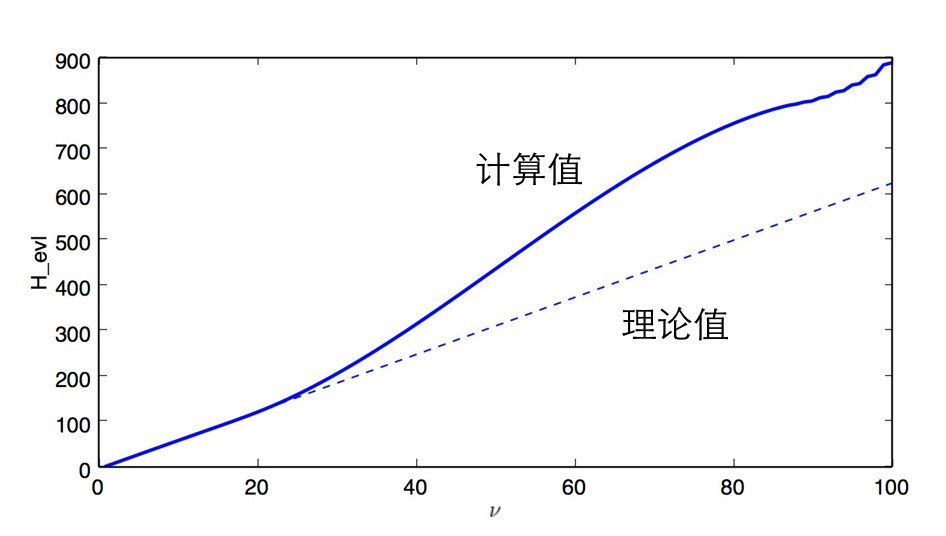
\includegraphics[width=0.99\linewidth]{H_err/H_err.pdf}
  \caption{\textbf{哈密顿量本征值计算结果的偏差} \label{fig:N_Hamiltonian}}
\end{figure}


\subsection{演化时间步长的影响}
注意到图\ref{fig:N_Cheby}(f)的异常情况,笔者怀疑是切比雪夫展开的数值方法在程序运行时发生崩溃,考虑到还有参数$dt$可以共同调节切比雪夫展开项的大小,改变时间步长并研究切比雪夫展开的性质可能可以支持之前的猜想。

全局演化方法处理含时演化算符在数学上的可行性是显然的:
\begin{IEEEeqnarray}{rCl}
  \Psi(t_1 + t_2) & = & \hat{U}(t_1 + t_2) \Psi(0)\nonumber \\
  & = & e^{(-i/\hbar)\hat{H}(t_1 + t_2)} \Psi(0)\nonumber \\
  & = & e^{(-i/\hbar)\hat{H}t_1} e^{(-i/\hbar)\hat{H}t_2}\Psi(0)\nonumber \\
  & = & \hat{U}(t_1) \hat{U}(t_2) \Psi(0) 
\end{IEEEeqnarray}
因此可以根据所需要演化的时间直接确定$dt$的值。无论是单步长步长演化还是多步短步长演化理论上结果是一样的。

在我们的简单模型中,理论与计算结果都表明直接对角化方法处理含时演化算符是可行的,在这里我们暂时不考虑效率的问题。对角化方法唯一依赖的参数是采样点数$N$,只要我们得到了哈密顿量的矩阵表示,所有剩下的问题只是将这个厄米矩阵对角化并求出特征向量和特征值。大量测试数据表明,对角化方法的演化结果和多步短步长切比雪夫演化结果一致性较高,图\ref{fig:Diag_evo} 是对角化方法单步和多步演化的结果,其中$\Psi(x) = 2 \sqrt[4]{2\pi^2}x e^{-\pi x^2 /10}$,参数为$N=250$,多步法中$dt=0.01$演化10步,单步法中$dt=0.1$,展开项数为。因此在切比雪夫展开和对角化方法的对比中,我们认为对角化方法的结果是近似准确的,并以此优化切比雪夫展开的参数设定。

\begin{figure}[hbt]
  \centering
  \captionsetup{justification=centering}
  \vspace{-1mm}
  \includegraphics[width=0.99\linewidth]{3.4/Diag.pdf}
  \caption{\textbf{对角化方法单步与多步演化结果} \\
            $\boldsymbol{\Psi(x) = 2 \sqrt[4]{2\pi^2}x e^{-\pi x^2 /10}}$}
  \label{fig:Diag_evo}
\end{figure}

接下来我们尝试切比雪夫展开的单步和多步演化,发现了其中的问题。我们发现使用小步长多次演化的结果与对角化演化的结果一致,然而大步长单词演化的结果有偏差。也就是说,使用我们的切比雪夫展开,初始体系一次演化10个单位时间的结果和进行10次单步演化的结果不一样,这显然是有悖常理的。图\ref{fig:Cheby_evo} 显示了这一错误结果。
\begin{figure}[hbt]
  \centering
  \captionsetup{justification=centering}
  \vspace{-1mm}
  \includegraphics[width=0.99\linewidth]{3.4/Cheby.pdf}
  \caption{\textbf{切比雪夫展开法单步与多步演化结果} \\
            $\boldsymbol{\Psi(x) = 2 \sqrt[4]{2\pi^2}x e^{-\pi x^2 /10}}$}
  \label{fig:Cheby_evo}
\end{figure}
既然多步演化给出的计算结果与对角化方法结果一直,我们姑且认为切比雪夫展开的理论推导与模型建立是正确的,那么问题只能出现在数值计算的过程中了。笔者仔细查看了程序中含时演化算符表达式(公式\ref{eq:cheby_equation} ),其中涉及$dt$项的只有相位调节因子$\beta$和系数$a_n$,其他诸如切比雪夫递归项中不涉及$dt$,因此确定了寻找问题的切入点。
\begin{equation*}
  \Psi(t) \approx e^{\beta} \sum_{n=0}^{N} a_n \phi_n[-i H_{\text{norm}}] \Psi(0)
\end{equation*}
在确认贝塞尔函数和递归函数的程序编写无误后,问题的矛头指向了切比雪夫展开项数。通过增加展开项数量,单步演化的结果成功收敛于期望值。在尝试增加展开项数的过程中,我们还发现$dt$的正加似乎会剧烈影响达到收敛的展开项数,为此我们制作了$dt$-收敛展开项数关系表,见表\ref{tab:dt-M}和图\ref{fig:dt-M},其中收敛的标准定位能量值精确到6位有效数字。由于不是精确的定量计算,我们只给出线性相关的结论而不给出具体的数值关系。
\begin{table}[hbt]
  \centering
  \begin{tabular}{|P{3.5cm}|P{3.5cm}|}
    \hline
    \multicolumn{2}{|c|}{N=250}\\ \hline
    $dt$ & 所需展开项数  \\ \hline
    0.01 & 40                    \\ \hline
    0.02 & 70                    \\ \hline
    0.05 & 160                    \\ \hline
    0.1 & 290                  \\ \hline
    0.15 & 430         \\ \hline
    0.2 & 560                  \\ \hline
  \end{tabular}
\captionof{table}{\textbf{$\boldsymbol{dt}$-展开项数关系}}
\label{tab:dt-M}
\end{table}

\begin{figure}[hbt]
  \centering
  \captionsetup{justification=centering}
  \vspace{-1mm}
  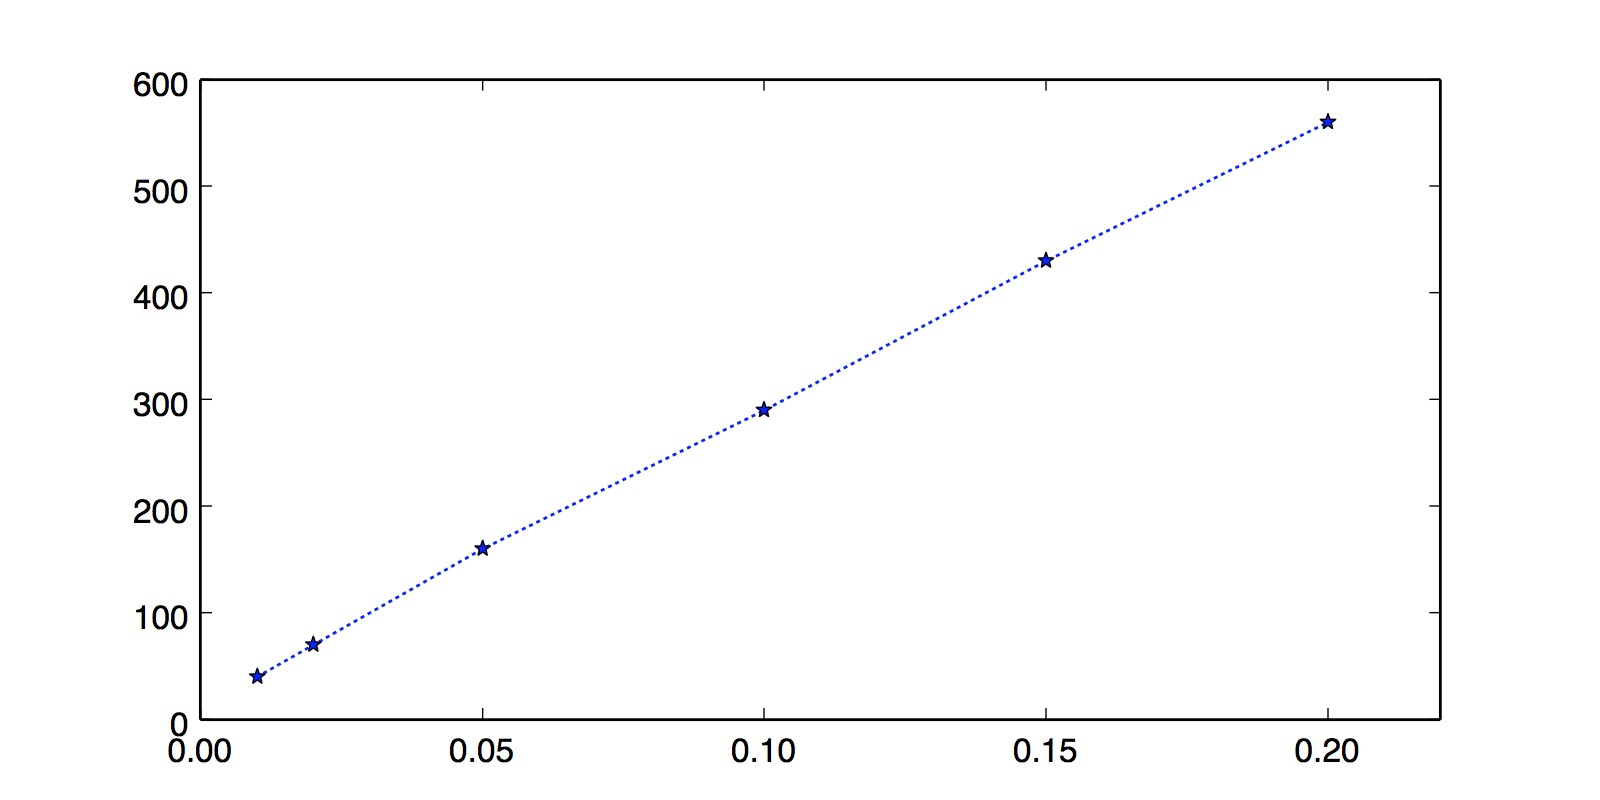
\includegraphics[width=0.99\linewidth]{dt-M/dt-M}
  \caption{$\boldsymbol{dt}$\textbf{与展开项数关系}}
  \label{fig:dt-M}
\end{figure}

可见随着时间步长的增长,所需要的切比雪夫多项式数量线性增长。我们手写的矩阵乘法的算法复杂度为$O(N^3)$,如果使用k步短步长演化,只需要将$\hat{U}$矩阵作用在波函数矢量上k次,即进行k次矩阵乘法;如果使用单步长步长演化,由于dt和展开项数的线性关系,相当于需要k倍的展开项系数才能构建$\hat{U}$,而每次递归循环中进行的复杂度最高的运算也是一次矩阵乘法,因此两种演化方法在复杂度上是相等的。

可以看出,在本课题所用模型中切比雪夫展开和对角化方法的表现较为一致。然而实际体系中切比雪夫展开的使用率要更高,最重要的原因在于其计算的误差被均匀分布于所有本征值中,并且计算的数值稳定性高。

\subsection{非定态本征态的含时演化}
前面我们已经看到,当含时演化算符作用在波函数定态本征态上,其概率分布不发生变化,这项结果是显然的:
\begin{equation}
  \Psi(t) = e^{(-i/\hbar)\hat{H}t}\Psi(0)
\end{equation} 
是含时薛定谔方程的解,从形式上看相当于在初始波函数前面加了一项复数系数,那么经过波函数归一化处理,其空间概率分布将不变。

如果初始状态为定态波函数的线性组合,例如:
\begin{equation}
  \left| \Psi(0) \right> = \alpha \left| \phi_1 \right> + \beta \left| \phi_2 \right>
\end{equation}
由于
\begin{IEEEeqnarray}{rCl}
  \left| \Psi(t)\right> & = & \alpha \left| \phi_1 \right> e^{-i\epsilon_1 t/\hbar} + \beta \left| \phi_2 \right> e^{-i\epsilon_2 t/\hbar} \nonumber \\
  i\hbar \frac{\partial}{\partial t} \left| \Psi(t)\right> & = & \alpha \epsilon_1 \left| \phi_1 \right> e^{-i\epsilon_1 t/\hbar} + \beta \epsilon_2 \left| \phi_2 \right> e^{-i\epsilon_2 t/\hbar} \nonumber \\
  & = & \hat{H} \left| \Psi(t) \right> \nonumber
\end{IEEEeqnarray}
所以
\begin{IEEEeqnarray}{rCl}
  \left| \Psi(t) \right> & = & \alpha \left| \phi_1 \right> e^{-i\epsilon_1 t/\hbar} + \beta \left| \phi_2 \right> e^{-i\epsilon_2 t/\hbar} \nonumber \\
  & = & e^{(-i/\hbar)\hat{H}t} \left| \Psi(0) \right> \nonumber \\
  & = & \hat{U} \left| \Psi(0) \right> \nonumber
\end{IEEEeqnarray}

当初始波函数不是演化算符中哈密顿量的本征态的时候,也是我们最常遇到的情况,就好像给初始的体系外加了一个势场,作用后可以得到演化后的波函数,这是我们构造含时演化算符的主要目的。如此一来给定体系的初始波函数后,通过作用含时演化算符得到以后任意时刻的波函数,那么就可以获得所有需要的信息。例如通过模拟一束激光作用在感兴趣的系统上,我们可以计算其拉曼光谱等。我们令

\begin{align*}
  \phi_1  &=  \sqrt[4]{2} e^{-\pi x^2} \\
  \phi_2  &=  2\sqrt[4]{2\pi^2} x e^{-\pi x^2}  \\
  \Psi(0)  &=  \frac{\sqrt{2}}{2}\phi_1 + \frac{\sqrt{2}}{2}\phi_2
\end{align*}
图\ref{fig:LC_Psi} 给出了其含时演化的结果。发现这个体系将做周期性的变化,用切比雪夫展开和对角化方法可以得到很接近的结果,不过我们还在试图找寻其他途径来证明我们的演化结果是正确的。
%\begin{figure}[hbt]
%  \centering
%  \captionsetup{justification=centering}
%  \vspace{-1mm}
%  \includegraphics[width=0.99\linewidth]{TBA}
%  \caption{$\Psi$随时间的演化情况}
%  \label{fig:LC_Psi}
%\end{figure}








\section{结论与展望}
\label{conclusion}
% !TEX root = Time_Evo.tex

本课题目前成功构建了以一维简谐振子模型为基础的含时演化算符,该算符适用于研究从给定的简谐振子初始状态到以后任意时刻的体系状态波函数演化的情况。在这里虽然我们使用的是简单的$sinc$函数作为基函数,并且在计算哈密顿量的数值方法中使用了三点近似和局部势能近似,但是从计算结果看来与理论预测相符。我们的目的并不是定量地准确研究体系的演化信息,而是尝试构造这样一个系统并用计算机程序从数值上实现它。从最终的程序运行结果来看本课题的模型构建较为成功,得到了我们想要的结果。

虽然本课题的量子化学理论背景并不深奥,主要涉及量子力学量在希尔伯特空间中的表示和含时演化算符的数值实现方法,但是理论学习和实际程序化是有差异的。在具体的构造过程中我们遇到了很多困难,例如:选取基函数时,既要满足能足够准确地展开波函数,又要满足正交归一的性质,还需要考虑边界条件和数值积分的稳定性。为了简易起见我们选用了$sinc$函数作为基函数,但是显然使用傅里叶级数的数值稳定性和算法效率都会更高,下一步我们将改用傅里叶级数为基函数。另外我们认为计算的误差来源还来自计算动能项中使用的三点近似方法,如果利用傅里叶变换理论上可以获得更高的精度,我们也考虑进一步优化动能项的算法。还有一方面的困难来自程序化方面,数值方法很多时候并不像理论那样可以给出很优美的解,数值计算可能会遇到一些意想不到的困难。

我们主要的研究对象--含时演化算符是含时方法的关键,例如我们想要研究关联函数$\left< \xi(0) | \hat{O} | \Psi(t') \right>$在任意时刻$t'$的信息,我们就可以将其展开为:
\begin{equation*}
  \left< \xi(0) \right| \hat{O} \left| \Psi(t') \right> \approx e^{\beta} \sum_{n=0}^N a_n \phi_n \left< \xi(0)\right| \hat{O} \left| \Psi(0) \right>
\end{equation*}
其中最常见的是偶极矩算符$\hat{\mu}$,通过对这些关联函数进行傅里叶变换我们可以模拟拉曼光谱等\cite{Raman}。如果条件允许我们也将进行光谱的模拟计算。

得益于计算机技术的高速发展,例如大规模并行化和量子计算机的问世,理论化学家可以研究的化学体系越来越复杂。含时量子力学方法在高性能计算的辅助下蓬勃发展,其高准确性、可移植性和高效性使它成为未来研究反应动力学和量子化学的利器。本课题模型的构建让我们得以管窥理论化学的宏伟体系。

\section*{\centerline{支持信息}}
% !TEX root = Time_Evo.tex

波函数含时演化相关程序源代码已上传至 \href{https://github.com/raymond931118/Time_Evolutionary_Wavepacket.git}{GitHub} (点击访问)。作者邮箱为\underline{yiqunwang2021$@$u.northwestern.edu} ,欢迎交流访问。

\section*{\centerline{致谢}}
\label{acknowledgement}
% !TEX root = Time_Evo.tex

本课题是加州大学洛杉矶分校Daniel Neuhauser教授为我设计的练习项目,为我步入量子化学的研究领域打下基础。承蒙我的导师-复旦大学李晔飞学者的悉心指导,我成功地用计算机程序实现了理论模型。还要感谢复旦大学刘智攀教授为我提供了工作场所和交流学术的环境,感谢张校捷学长长期提供学术咨询。


\begin{spacing}{1}
  \wuhao
  \bibliographystyle{IEEEtranN}
  \bibliography{refsc}
\end{spacing}

\end{document}
